% Metódy inžinierskej práce

\documentclass[12pt,twoside,english,a4paper]{article}

\usepackage[english]{babel}
%\usepackage[T1]{fontenc}
\usepackage[IL2]{fontenc} % lepšia sadzba písmena Ľ než v T1
\usepackage[utf8]{inputenc}
\usepackage{graphicx}
\usepackage{url} % príkaz \url na formátovanie URL
\usepackage{hyperref} % odkazy v texte budú aktívne (pri niektorých triedach dokumentov spôsobuje posun textu)
\usepackage{float}

\usepackage{cite}
%\usepackage{times}

\pagestyle{headings}

\title{The development of Dota 2, features of the game\thanks{Semestrálny projekt v predmete Metódy inžinierskej práce, ak. rok 2022/23, vedenie: Vladimír Mlynarovič}} % meno a priezvisko vyučujúceho na cvičeniach

\author{Khrystyna Bindiuk\\[2pt]
	{\small Slovenská technická univerzita v Bratislave}\\
	{\small Fakulta informatiky a informačných technológií}\\
	{\small \texttt{xbindiuk@stuba.sk}}
	}

\date{\small 4. november 2022} % upravte



\begin{document}

\maketitle

\begin{abstract}

Nowadays computer games are widely used by various age groups ranging from children to adults. A majority of users prefer the genre of action games. One of the most popular action games is Dota 2 in accordance with an ongoing analysis of Steam's concurrent players. As a consequence, the main purpose of the article is to describe the phases of Dota 2 development, the main features of the game, and the factors that caused its popularity. The paper consists of several parts such as the development phases of Dota 2, the main features of Dota 2, and the reasons why Dota 2 is still popular.
\end{abstract}



\section*{Introduction}

Computer games become indispensable parts of daily lives in recent decades. It is caused by the global digitalization of society and the irreversible penetration of state-of-the-art technologies into the market. As a result, there is a growing demand for products that may capture the attention of possible users. To achieve the above-mentioned goal, game developers introduce fresh and unusual scenarios and heroes in their programs. One of those games is Dota 2. 

Dota 2 is a multiplayer online battle arena game that was created by the American video game developer company Valve Corporation. The product is known for its isometric perspective, 3D graphics and wide range of modes. Moreover, players have the possibility to choose various heroes because there are 123 characters that users can take from before the beginning of a battle.

The article covers the phases of Dota 2 development in the section~\ref{The development phases of Dota 2}. Furthermore, the main characteristics of the game and factors that have an impact on Dota 2 popularity are described in~\ref{The main features of Dota 2} and~\ref{the reasons why Dota 2 is still popular}. The concluding remarks are provided in the part~\ref{conclusion}.



\section{The development phases of Dota 2} \label{The development phases of Dota 2}
It is claimed that the development path of Dota 2 consists of several phases.

First and foremost, the concept of the game originated from the Aeon of Strife fan mod for StarCraft: Brood War in 1998\cite{Stubbs:Rise}. The interesting point in the Aeon of Strife is that the three-lane system of creeps was the impetus for the development of Dota 2. 

Moving forward, modder Kyle “Eul” Sommer created a mod for Warcraft 3 called Defense of the Ancients or DotA in the early 2000s. The main difference with the modern mod of Dota 2 is an engine that misses bells and whistles. Other features are similar to Dota 2. To some extent, there are five players per team that compete against five others on a map with three lanes and try to destroy the base of an opposite team. At the same time, each unique character has distinguishable abilities and properties. 

Next, new versions of the mod appeared because the code of the map was opened for everyone. One of the most popular among them was Dota Allstars\cite{Pra:What} which was developed by Steve “Guinsoo”. Therefore, Dota Allstars became the prototype of Dota 2.

Finally, Valve Corporation decided to work on a project with game developer IceFrog in 2009. The game was released in beta form in 2011 and gained popularity among players from around the globe. Later, it was officially published on Steam in mid-2013. In addition, in 2015 there was a “Reborn” update that completely changed the User Interface of the game. The next update called the 7.00 update was in 2016, and it is regarded as the greatest transformation of core Dota 2 gameplay.




\section{The main features of Dota 2} \label{The main features of Dota 2}


Dota 2 is known for its huge range of features. Thus, the section is divided into an overview of Dota 2~\ref{overview}, its main modes~\ref{main modes}, positions~\ref{positions} and heroes~\ref{heroes}. 


\subsection{An overview of Dota 2} \label{overview}


Each team has five players. If a team invades the opponent’s base and destroys the Ancestor, it is considered a victory. Each player has a specific position and one person is designated as captain. The captains of each team have the possibility to choose five heroes, who will be in their team. During the draft, a captain can ban some heroes from usage by opponents. Then, team members select heroes from remained options. When a person chooses a character, he needs to pay attention to the individual strengths and weaknesses of it as well as the strengths and weaknesses of that hero in combination with characters already selected by other team members\cite{Conley:Dota}. 

Furthermore, an economic system is available in the game. To explicate, a user can earn gold when he kills a creep of another team. Therefore, if a player wants to become stronger, he needs to earn more gold and buy special items that boost a hero.
In Dota 2, there are also “neutral creeps” which are outside of the lanes and forest monsters. An interesting aspect of the game is a creature called “Roshan” who is capable of changing fate. After a player killed Roshan, he gets the item that can revive a person after death.



\subsection{Main modes} \label{main modes}

There are several main modes in Dota 2 such as captains mode, random draft, turbo, least played, limited heroes, 1v1 solo mid, all random deathmatch, ability draft and single draft.
\begin{figure}
  \centering
  \caption{Main modes of Dota 2\cite{ Modes:Nathan}}
  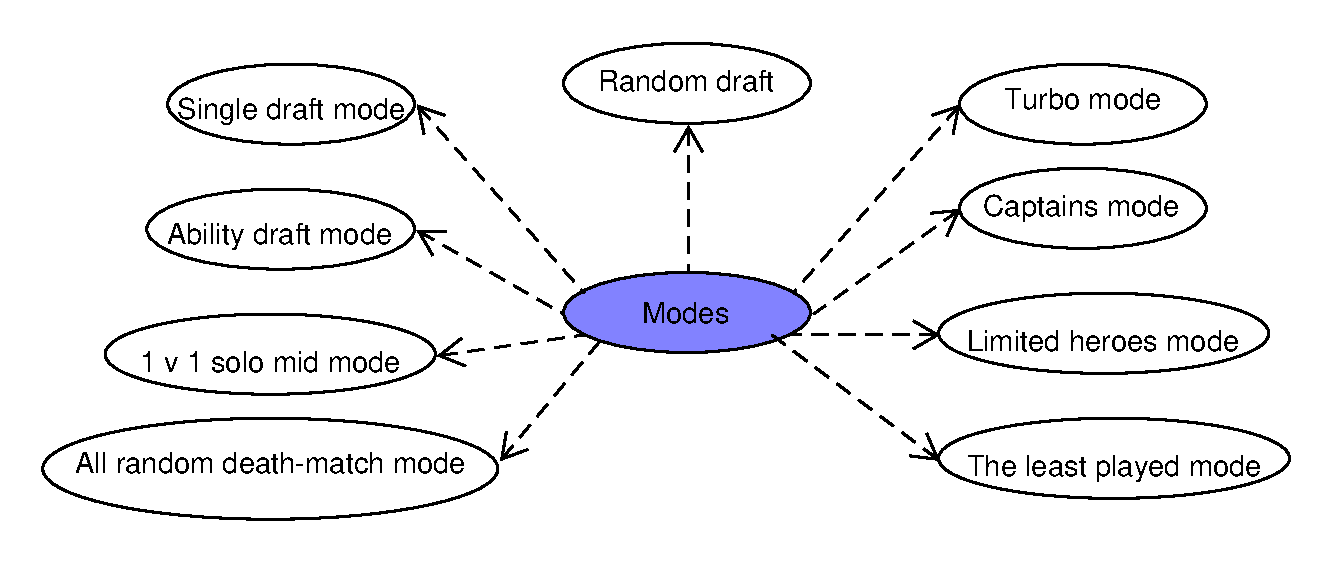
\includegraphics[width=1.0\textwidth]{modes123094.pdf}
  \label{fig:modes}
\end{figure}  

Captains mode is used mainly for tournament games. The captains are able to ban heroes, up to seven per team, for the opponent. After the captains’ selection, each team member picks up a character. Also, a captain has 130 bonus seconds. 

A random draft is a mode when team members take turns after they chose heroes.

Turbo mode distinguishes by its quick drafting, doubled experience gain, fast dropping of all tiers, quick couriers and fast upgrade of lane creeps.

In the least played mode, a player can not pick up any of his 40 most used characters.

Limited heroes mode proposes a heroes pool that is designated for beginners.

1 v 1 solo mid mode gives a user a chance to compete against another player. A person who has two kills or destroys an enemy tower faster wins.

At the beginning of a battle in all random deathmatch mode, every team member has a random hero. After death, a player receives a new random hero upon respawning. There are only 40 respawns per team. 

Ability draft mode enables a player to choose three normal abilities and one ultimate for his hero.

In single draft mode, a user picks up three random heroes from a pool.

\subsection{Positions} \label{positions}
There are five basic positions in Dota 2.\cite{ Balaji:Dota}

\textbf{Position 1: Carry/Safe-lane} (Medusa, Anti-mage, Juggernaut)

The first position is the hero called the carry-player or safe lane. 
His responsibility is to get gold and experience. At the beginning of a battle, he is weaker than a support player in fights. To get farm and levels, he usually needs to be protected by all the other heroes on your team for the first 10 minutes. It usually takes the first ten minutes for him to get levels. At this time, the protection of other heroes is essential for a safe lane. When a carry player reaches a farm and levels, he can alone kill 2 opponents.

\textbf{Position 2: Mid-lane}      (Invoker, Templar Assassin, Shadow Fiend)
Midlane is a player who fights alone. In this way, he gains experience the fastest among other heroes. A character can amplify farms and get early kills on the side lanes.

\textbf{Position 3: Off-lane }(Axe, Tidehunter, Underlord)
The off-lane chases the enemy carry player and expands the map for other team members.

\textbf{Position 4: Roaming Support    } (Spirit Breaker, Earth Spirit)                            
The main task of the roaming support is to make rotations to other lanes and to try to make kills. This kind of hero can not go to the forest. Meanwhile, roaming support is able to affect various routes.

\textbf{Position 5: Hard Support}       (Crystal Maiden, Lion, Witch Doctor)            
Hard Support provides the security of a carry hero against the off-lane and roaming support.
\subsection{Heroes} \label{heroes}
Dota 2 has 123 heroes. The newest of them is Primal Beast. Most of these heroes have prototypes from the first Defense of the Ancients. However, some heroes, such as Monkey King and Mars, are entirely new heroes not found in the original version of Dota 2.
Heroes have one of three primary attributes: Strength, Agility, and Intelligence. Every point of a hero's primary attribute increases that hero's attack damage.
 \begin{figure}[H]
  \centering
  \caption{Attributes table of heroes in Dota 2\cite{Heroes:DOTA}}
  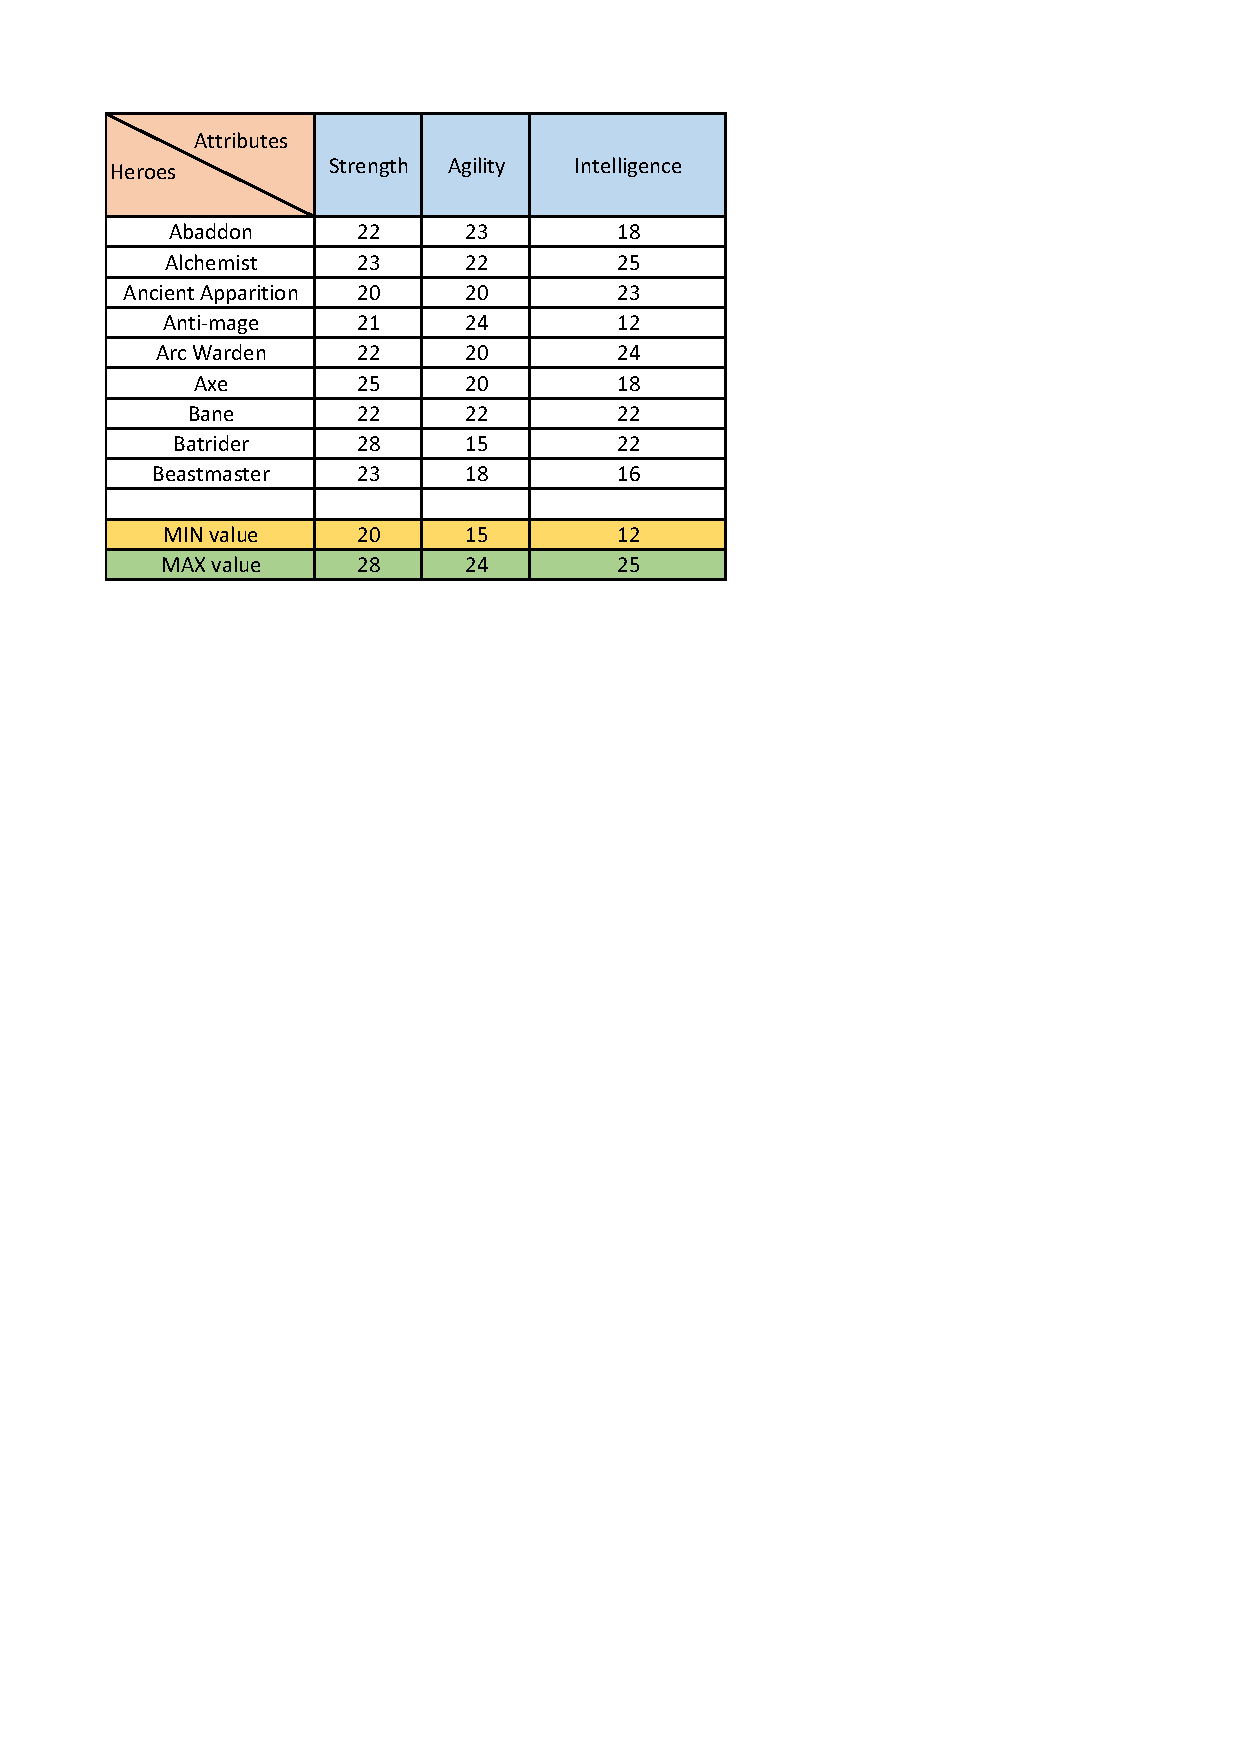
\includegraphics[width=0.8\textwidth]{heroes123094.png}
  \label{fig:heroes}
 \end{figure}  
\section{The reasons why Dota 2 is still popular} \label{the reasons why Dota 2 is still popular}
There are several reasons why Dota 2 is still popular among players. First of all, the game proposes a huge variety of heroes, items, and upgrades that helps to capture the attention of users. Secondly, Dota 2 is mainly free. In this way, it is available for a majority of people. Thirdly, championships and various competitions are organized every year. Therefore, every player has an opportunity to experience eSports by being an eSports player.\cite{Reasons:DOTA}
\section{Conclusion} \label{conclusion} % prípadne iný variant názvu
Currently, the popularity of Dota 2 is growing considerably among players. The development process of the action game consists of several phases, commencing with the Aeon of Strife fan mod and ending with the official game release in 2013. Furthermore, the main reason for users’ interest in Dota 2 is its wide range of features, such as a variety of main modes and heroes for five positions. 



%\acknowledgement{Ak niekomu chcete poďakovať\ldots}

\paragraph{Technology and people}
Technology is a powerful tool that may meet people's needs. One of them is to organize group work to achieve tangible results. As a result, Agile appeared as a framework for project realization. There are four core values of Agile. The first one is that individuals and interactions are over processes and tools. Next, working software is over comprehensive documentation. The third principle is that customer collaboration is over contract negotiation. The last notion is that responding to change is over following a plan.

Moreover, one of the most popular methodologies of software development is Scrum. It is based on six principles. The first idea is that empirical process control helps to learn through experimentation. Furthermore, the second principle is that self-organization is crucial for better team buy-in and shared ownership. The next notion is that project delivery is a shared value-creation process with teams working and interacting. The fourth statement is to deliver maximum business value from the beginning of the project to the end of it. The following principle is that time is a limiting constraint in Scrum and is used to manage project planning and execution. The last idea is based on iterative development that helps to create programs effectively.
\paragraph{History of Informatics}
The history of Informatics consists of several phases.

To begin with, the earliest known tool in computation was the abacus, which was created in Sumer. Next, the Antikythera mechanism was designed to calculate astronomical positions. This device is believed to be an early mechanical analog computer. Later, Muslim engineers invented programmable machines, such as Al-Jazari's programmable castle clock, which is considered to be the first programmable analog computer. In 1702, Gottfried Wilhelm Leibniz developed the binary numeral system. Beginning in the 1810s, Babbage designed a calculator to compute numbers up to 8 decimal points long.

Furthermore, the mathematical foundations of modern computer science were laid by Kurt Gödel in 1931. In 1936 Alan Turing and Alonzo Church introduced the formalization of an algorithm, with limits and a "purely mechanical" model for computing. Claude Shannon published A Mathematical Theory of Communication in 1948, which applied probability theory to the problem of how to best encode the information that will be transmitted. 
\paragraph{Sustainability and ethics}
It is essential to provide sustainable development which means that resources can be restored or even before theirs through exhaustion they would be replaced with alternative sources. To achieve this kind of development, a person should personally internalize the belief, persuade others to take over responsibility for one's actions, use resources more efficiently, recycle, turn off what he can and use what cannot be turned off.

There is a Software Engineering Code of Ethics that has eight principles. The first principle claimed that software engineers shall act consistently in the public interest. The second one said that programmers ought to act in a manner that is in the best interests of their clients and employer and consistent with the public interest. The third principle is based on the idea that developrs shall ensure that their products and related modifications meet the highest professional standards possible. The fourth notion is that coders ought to maintain integrity and independence in their professional judgment. The fifth claim is that software engineering managers and leaders shall subscribe to and promote an ethical approach to the management of software development and maintenance. The sixth principle is that pragrammers shall advance the integrity and reputation of the profession consistent with the public interest. The seventh idea is that coders shall be fair to and supportive of their colleagues. The last notice is that software engineers shall participate in lifelong learning
regarding the practice of their profession and shall promote an ethical approach to the practice of the profession.

% týmto sa generuje zoznam literatúry z obsahu súboru literatura.bib podľa toho, na čo sa v článku odkazujete
\bibliography{literatura}
\bibliographystyle{plain} % prípadne alpha, abbrv alebo hociktorý iný
\end{document}
